\chapter{Details of Virtual Memory subsystem}
\label{chapter:details}

In this chapter, we will look at the details of UVM, the virtual memory implementation created by Charles D. Cranor
and originally used in the NetBSD operating system \cite{cranor}.
It was designed to improve performance of virtual memory subsystem and to implement new features that were impossible to express using the old VM system.
The description of UVM here will give the details of fully working implementation in NetBSD.
The details of the implementation of UVM in Mimiker are in chapter~\ref{chapter:mimiker}.
It is essential to dive into the details of the model implementation of UVM to understand the part of it created in Mimiker.
The implementation in Mimiker is also not complete yet so this chapter will describe some features and mechanisms still not supported.
They are not yet present in Mimiker, because it would require to review and modify many other subsystems,
such as Virtual File System or interface between kernel and memory devices.

The code snippets used in this chapter are from the NetBSD sources \cite{netbsd:sources}.
To improve readability, non-essential fields have been removed from the code listings for easier analysis.

\section{Memory map of the process}

The operating system kernel must have full knowledge of the process' virtual memory map.
On the figure~\ref{img:typical-vm-map}, there is a part of typical memory map of the process.
All structures presented on that figure are used to handle all memory-related operations requested by the process.
Later in this chapter we will see all these structure in details:

\begin{samepage}
\begin{itemize}
  \item \mintinline{c}{vm_map} -- high-level description of process memory map
  \item \mintinline{c}{vm_map_entry} -- describes an individual memory segment
  \item \mintinline{c}{vm_amap} -- used to describe anonymous memory used within single segment
  \item \mintinline{c}{vm_object} -- represents a resource mapped as a memory segment (usually~a~file)
  \item \mintinline{c}{vm_aref} -- reference to an amap structure
  \item \mintinline{c}{vm_anon} -- describes a single page of anonymous memory
  \item \mintinline{c}{vm_page} -- describes a single physical page
\end{itemize}
\end{samepage}

\begin{figure}
  \centering
  \includegraphics[width=0.8\textwidth]{typical-map.png}
  \caption{Part of typical virtual memory map of the process}
  \label{img:typical-vm-map}
\end{figure}

On the top level two structures are used: \mintinline{c}{vm_map} and \mintinline{c}{vm_map_entry}.
These structures are used to properly define and manage the memory segments used by the process.

The \mintinline{c}{vm_map} stores the list of memory segments and a reference to page table structure that describes physical mappings -- \mintinline{c}{pmap}.
The \mintinline{c}{pmap} reference is used to update the mappings from virtual to physical addresses after an operation is performed on the virtual memory.
When performing an operation on the VM~map, the list of entries is usually traversed to find, insert or remove a segment.
To perform any operation on the list of segments, the VM~map lock must be held.

For the details of the VM~map structure, see the listing~\ref{code:vm_map}.

\begin{listing}
  \begin{minted}{c}
struct vm_map {
    krwlock_t lock;             /* VM map lock */
    int flags;                  /* Flags */
    struct pmap *pmap;          /* Physical map */
    int nentries;               /* Number of entries */
    struct vm_map_entry header; /* List of entries */
};
  \end{minted}
  \caption{VM~map structure}
  \label{code:vm_map}
\end{listing}

Each segment is described by a single structure -- \mintinline{c}{vm_map_entry}.
Conceptually, the VM~map entry is just a collection of pages that form a described memory segment.
Although, to make all operations on the memory more efficient a few different structures are used to maintain all the underlying pages.

The most important parts of VM~map entry structure are:

\begin{itemize}
  \item Address range -- the portion of memory that is described by this segment.
  \item Protection attributes -- the types of access allowed to the memory described by this segment.
  \item Segment flags -- the type of the segment (private or shared).
    and other attributes that define the type of memory it describes and how it must be managed (e.g. CoW segment).
  \item VM object and amap -- the structures that are used to manage the pages of the memory represented by the segment.
\end{itemize}

VM~map entries reference two types of objects that are used to store memory pages (UVM~objects and amaps)
because they are used to represent different types of memory.
Amaps describe anonymous memory, and UVM~objects represent the memory mapped files.
They create two level structure which is respected during a page lookup done during page fault.
If amap exists for a given VM~map entry, then it is the first to be searched.
Otherwise, or when page is not found in the amap, it is looked for in the UVM~object.
Amap is usually called a {\it shadowing layer} for the UVM~object.
If some page exists in both structures, its version stored in amap shadows the version from UVM~object.
This means that the version found in amap is always used to store the most recent data.
The attributes of the VM~map entry can be seen in details on listing~\ref{code:vm_map_entry}.

\begin{listing}
  \begin{minted}{c}
struct vm_map_entry {
    uint8_t flags;              /* flags */
    vaddr_t start;              /* start address */
    vaddr_t end;                /* end address */
    voff_t offset;              /* offset into object */
    vm_prot_t protection;       /* protection code */
    vm_inherit_t inheritance;   /* inheritance */
    struct uvm_object *uvm_obj; /* uvm object */
    struct vm_aref aref;        /* anonymous overlay */
};
  \end{minted}
  \caption{VM~map entry structure}
  \label{code:vm_map_entry}
\end{listing}

\section{The role of the amaps}

Anonymous memory is the memory that is released when it is no longer referenced (e.g. it has been unmapped by all processes that were using it),
because it isn't associated without any named resource like a file or device memory.
One possibility to create an anonymous memory mapping is to request one from the OS kernel using a \mintinline{c}{mmap} call.
In this case the map entry describing the requested segment contains only the reference to the amap.

The other option to create an anonymous mapping is to modify a memory in privately mapped file or other resource.
In such case, the changes made to the memory cannot be seen outside the process memory.
When the process writes to the memory page, which had to be fetched using the UVM~object, it has to be copied to the amap layer.
Because the amap layer is searched before the UVM~object, any lookups of that page will find the copy of it stored in the amap.
This ensures that all modified pages of private mappings are stored only in amaps and are freed after they are no longer in use.

\subsection{Referencing amaps from \mintinline{c}{vm_map_entry}}

Sometimes \mintinline{c}{vm_map_entries} are split into many parts
(e.g. when \mintinline{c}{mprotect} is called on a fragment of the segment to change its access protection).
After splitting, each created VM~map entry must point to a specific fragment of the original amap.
Instead of creating new amaps with content copied from the previous one, the amaps are referenced with a \mintinline{c}{vm_aref} structure.
It is a part of the \mintinline{c}{vm_map_entry} structure, and makes it possible to reference a part of the amap, specified by the offset.
If the VM~map entry is split into multiple entries, each part of it references the same amap but with different offsets.

The \mintinline{c}{vm_aref} structure is presented on listing~\ref{code:vm_aref}
and the usage of arefs during the amap split operation is pictured on the figure~\ref{img:amap_split}.

\begin{listing}[h]
  \begin{minted}{c}
struct vm_aref {
  size_t offset;
  struct vm_amap *amap;
};
  \end{minted}
  \caption{Aref structure}
  \label{code:vm_aref}
\end{listing}

\begin{figure}[h]
  \centering
  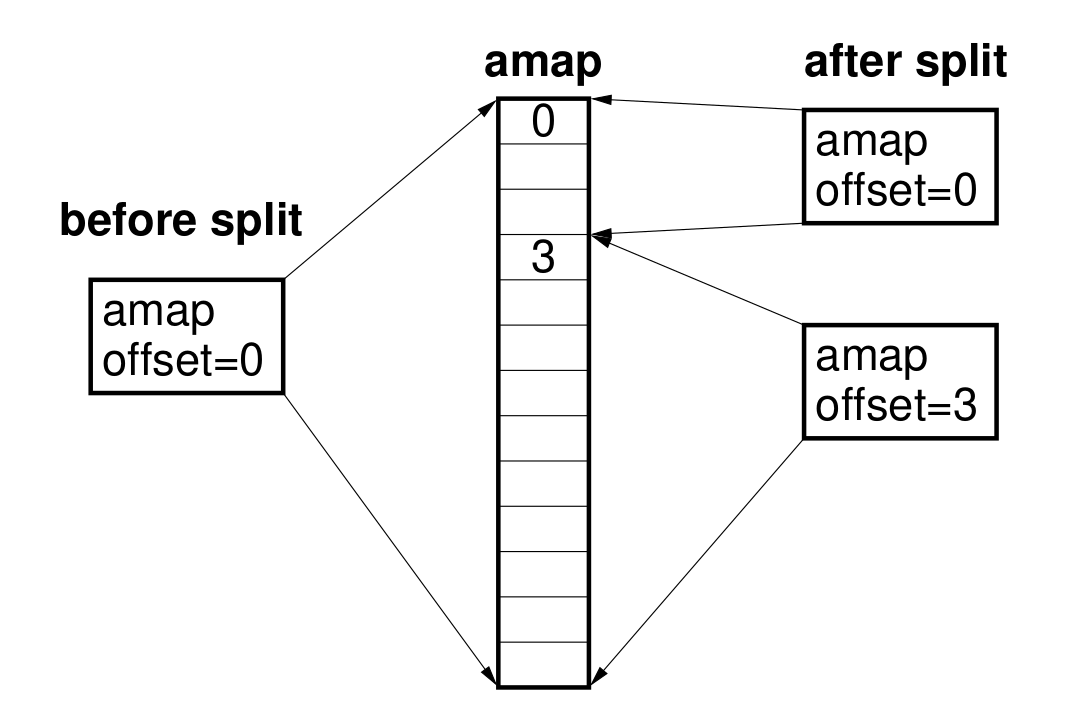
\includegraphics[width=0.5\textwidth]{amap-split.png}
  \caption{Illustration of the split of an amap \cite{cranor}}
  \label{img:amap_split}
\end{figure}

\subsection{Representing anonymous memory pages}

Individual pages of anonymous memory are described using a dedicated \mintinline{c}{vm_anon}, structure sometimes referred to as anon (listing~\ref{code:vm_anon}).
Its purpose is to make it possible to share pages between multiple amaps.
Anon structure keeps track of the number of amaps that are referencing it, in order to free the page when it is not referenced anymore.

Anons can describe resident pages as well as swapped out ones.
The pages that are already in the main memory are referenced using the \mintinline{c}{page} field.
For the pages in the backing storage the \mintinline{c}{swap_slot} number is used to retrieve them from it when they are needed again.

\begin{listing}[h]
  \begin{minted}{c}
struct vm_anon {
    krwlock_t *an_lock;      /* Lock for an_ref */
    uintptr_t an_ref;        /* Reference count [an_lock] */
    struct vm_page *an_page; /* If in RAM [an_lock] */
    int an_swslot;           /* If in swap */
};
  \end{minted}
  \caption{Anon's structure}
  \label{code:vm_anon}
\end{listing}

\subsection{Basic implementations of amaps}

Amaps store anons that represent pages that have been allocated and accessed by the process.
References to them are stored in some data structure, and single reference is saved in an {\it amap slot}\footnotemark.
\footnotetext{
  Amap slots are entirely different concept than the backing storage slots.
  Thy describe the location of anons and are used to represent location of the anon in virtual memory address space.
  In contrast, backing storage is used to store raw content of memory pages that were swapped out.
  The swap slot number, which is recorded in the anon structure, is the location of memory of given page in the backing storage.
}
Slots may be active, when they have valid reference to an anon, or inactive, when they don't hold any anon.
Typically, amap slots are inactive if the portion of memory that would have been described by the anon referenced by the given slot
is described by the UVM~object or hasn't been accessed by the process yet.
We access individual slots using the index ({\it slot number}),
which is calculated from the virtual address of the memory that is within the range represented by the given amap.

Operation on amaps are performed using amap API, which makes it possible to provide different implementations of amaps.
When adjusting the OS kernel to run on some constrained machine, the most efficient implementation may be chosen.
Later we will see three different implementations of amaps.

The most important operations defined in the amap API:

\begin{itemize}
  \item \mintinline{c}{amap_alloc} and \mintinline{c}{amap_free} -- allocate new amap and free one
  \item \mintinline{c}{amap_ref} and \mintinline{c}{amap_unref} -- increase and decrease reference count of the amap
  \item \mintinline{c}{amap_extend} -- increase the size of amap
  \item \mintinline{c}{amap_add} and \mintinline{c}{amap_unadd} -- add and remove anons from amap
  \item \mintinline{c}{amap_lookup} -- search for anon
  \item \mintinline{c}{amap_copy} -- make a shallow copy of the amap (anons are not copied, but referenced from both original and new amaps)
  \item \mintinline{c}{amap_cow_now} -- make a deep copy the amap (every anon referenced from the amap is also copied)
\end{itemize}

The two basic implementations, array-based and list-based, are described below.
They are also presented on figures \ref{img:array-amap} and \ref{img:list-amap}.

\subsubsection{List based amaps}

This implementation uses a list to store references to \mintinline{c}{vm_anon} structures.
It will use exactly as many slots as needed, so it could be used if the system is running on a memory-constrained device.
Mass operations on the anons stored in the amap are fast
(looping through the list is efficient, because all visited list elements represent the anons that are actually being used).
On the other hand, operations on individual anons can be slower (finding a specific anon in the list requires iterating over the whole list).

\subsubsection{Array based amaps}

This implementation stores pointers to \mintinline{c}{vm_anon} structures in the array indexed by the slot number.
It also keeps track of active slots (the slots that hold already used anons).
Here, operations on single anons are fast (knowing the offset of the anon allows to get it instantly from the array).
Iterating over all active anons is now slower, because all slots have to be checked.

\begin{figure}
  \centering
  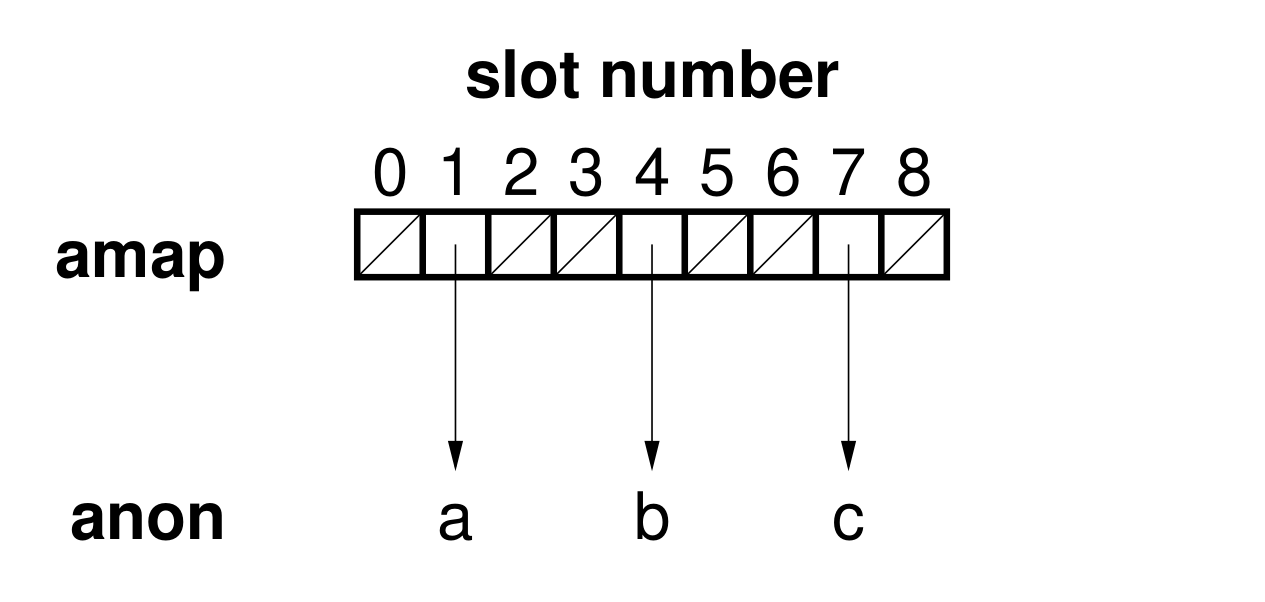
\includegraphics[width=0.5\textwidth]{array-amap.png}
  \caption{Amap implementation with an array of anons \cite{cranor}}
  \label{img:array-amap}
\end{figure}

\begin{figure}
  \centering
  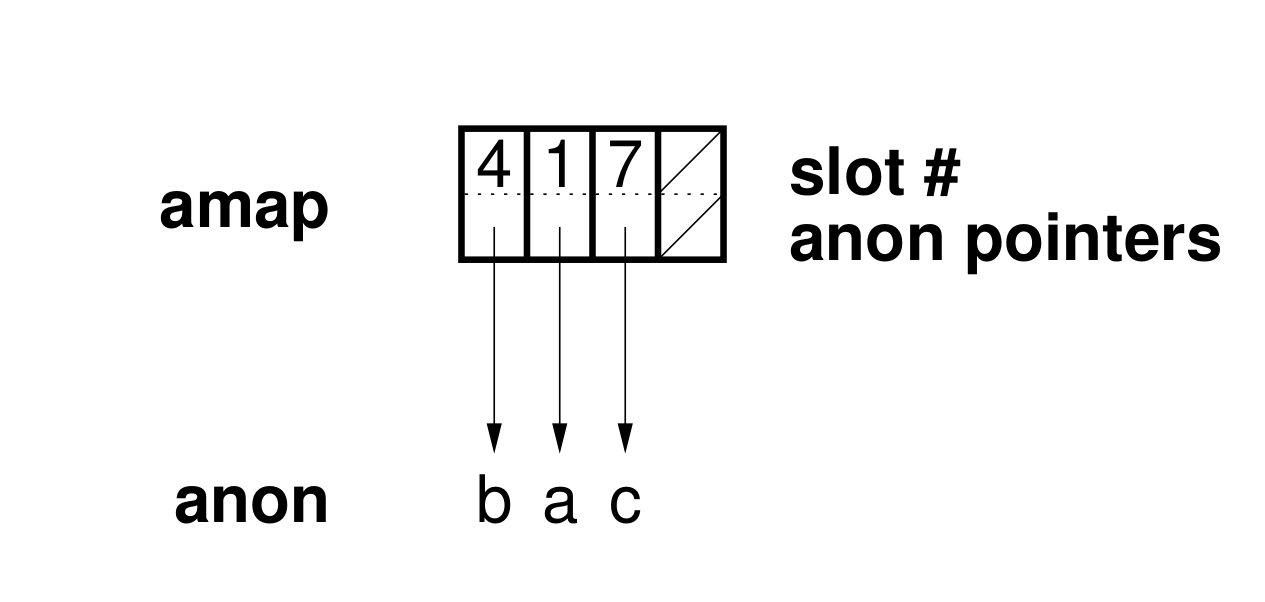
\includegraphics[width=0.5\textwidth]{linked-list-amap.png}
  \caption{Amap implementation with a list of anons \cite{cranor}}
  \label{img:list-amap}
\end{figure}

\subsection{Implementation of amaps used in UVM}

Both of the above implementations of amaps are good at one type of operation, but slow at others.
UVM uses a different approach.
It combines both implementations to create a one that is efficient in all types of operations.
The disadvantage is that it uses more memory (it needs 3 arrays instead of 1).

\mintinline{c}{vm_anon} structures are stored in the array indexed by slots (\mintinline{c}{am_anon}).
Slot numbers of active anons are stored in the list (\mintinline{c}{am_slots}).
To synchronize these structures the third one (\mintinline{c}{am_bckptr}) is used.
For each active slot, it stores its position on the list.
It is used to update the list of active anons when an anon is deleted.
The relations between all these three arrays are presented on figure~\ref{img:uvm_amap_impl}
and the C structure that describes the amap is on the listing~\ref{code:vm_amap}.

\begin{figure}
  \centering
  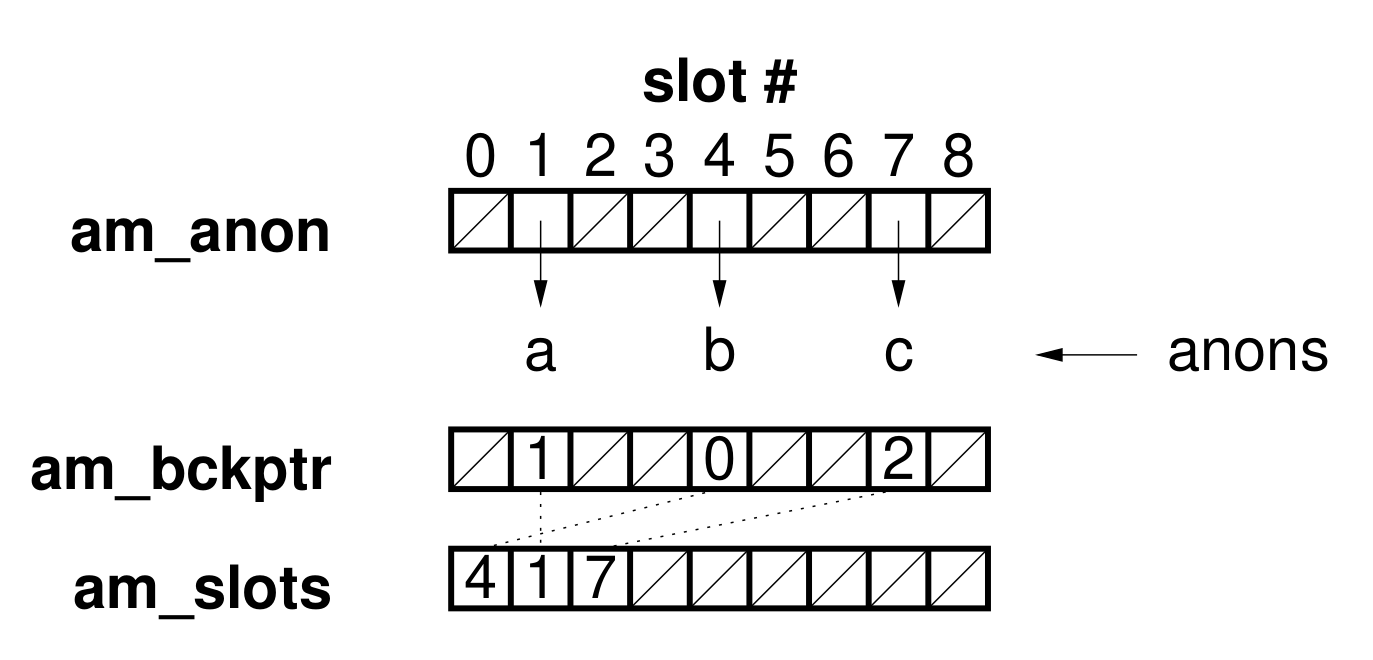
\includegraphics[width=0.5\textwidth]{uvm-amap.png}
  \caption{Amap implementation used in UVM \cite{cranor}}
  \label{img:uvm_amap_impl}
\end{figure}

\begin{listing}
  \begin{minted}{c}
struct vm_amap {
    krwlock_t *am_lock;       /* lock [locks all vm_amap fields] */
    int am_ref;               /* reference count */
    int am_flags;             /* flags */
    int am_maxslot;           /* max # of slots allocated */
    int am_nslot;             /* # of slots currently in map  */
    int am_nused;             /* # of slots currently in use */
    int *am_slots;            /* contiguous array of active slots */
    int *am_bckptr;           /* back pointer array to am_slots */
    struct vm_anon **am_anon; /* array of anonymous pages */
};
  \end{minted}
  \caption{Amap structure}
  \label{code:vm_amap}
\end{listing}

\begin{samepage}
\section{The role of the UVM~object}

Memory segments in the VM~map of the process may also represent the memory of files and devices.
To properly manage them and keep in sync with the actual memory of the resources there is a need for another structure.
  UVM~object structure, presented on listing~\ref{code:uvm_object}, holds three types of information:

\begin{itemize}
  \item A structure to keep track of the pages that are resident, along with a total number of them (\mintinline{c}{uo_npages} and \mintinline{c}{uo_pages}).
  \item The number of references from VM~map entries to that object (\mintinline{c}{uo_refs}).
  \item The reference to pager operations for given type of UVM~object (\mintinline{c}{pgops}).
\end{itemize}

\end{samepage}

\begin{listing}[h]
  \begin{minted}{c}
struct uvm_object {
    struct krwlock *vmobjlock;  /* lock on object */
    int uo_npages;              /* # of pages in uo_pages */
    unsigned uo_refs;           /* reference count */
    struct radix_tree uo_pages; /* tree of pages */
    const struct uvm_pagerops *pgops; /* pager ops */
};
  \end{minted}
  \caption{UVM~object structure}
  \label{code:uvm_object}
\end{listing}

UVM~objects represent the memory of some resource, hence they need to reference that resource in some way.
Instead of using dedicated structure field to record that the author of UVM decided to express it differently.
Every resource that can be mapped into process's memory has an UVM~object structure embedded into its structure.
As a result, knowing what type of resource is connected with given UVM~object we can calculate the address of that resource, based on the address of UVM object.
Actually, to make it even more direct, the UVM~object is saved at the beginning of the structure (as its first field).
On listing~\ref{code:vnode} there are a few initial lines of \mintinline{c}{struct vnode} definition, that shows the inclusion of UVM~object into vnode structure.

\begin{listing}[h]
  \begin{minted}{c}
struct vnode {
    struct uvm_object v_uobj;
    voff_t      v_size;
    /* Other fields ... */
};
  \end{minted}
  \caption{Part of the \mintinline{c}{vnode} structure}
  \label{code:vnode}
\end{listing}

\subsection{Pager interface}

Pagers define how operations are made on different types of UVM~objects.
The operations possible to perform are described by the {\it pager interface}, but each pager type provides its own implementation of them.
There is exactly one pager defined for each type of UVM~objects, and they are initialized during a system startup.
Every UVM~object references one structure which has the references for pager operations suitable for object of given type.
Because all operations on UVM~objects are conducted via the pager interface, there is no need to explicitly save the type of UVM object inside its structure.
By referencing a set of dedicated pager operations, the proper implementation of requested operation is executed.

Operations defined in the pager interface:
\begin{itemize}
  \item \mintinline{c}{pgo_init}
    -- Initialize the pager private data structures (e.g. the linked list of all allocated device-backed objects).
       Used only once for each pager during boot.

  \item Attach operation used during the creation of UVM~object.
    -- Each pager type defines its own attach function which performs all actions needed to obtain UVM~object of given type.
       (E.g. \mintinline{c}{uao_create} -- for anonymous UVM~objects,
             \mintinline{c}{udv_attach} -- for device-backed UVM~objects, and
             \mintinline{c}{uvn_attach} -- for vnode UVM~objects.)

  \item \mintinline{c}{pgo_reference}
    -- Increase reference count of the object.

  \item \mintinline{c}{pgo_detach}
    -- Decrease reference count of the object.

  \item \mintinline{c}{pgo_get}
    -- Get page from the object or read it from the backing storage.
       Typically called during page fault.

  \item \mintinline{c}{pgo_fault}
    -- Custom fault processing routine used when \mintinline{c}{pgo_get} isn't enough.

  \item \mintinline{c}{pgo_put}
    -- Write dirty page to the backing storage.
       Usually performed by the page daemon.

\end{itemize}

\subsection{Pager types}

UVM~object are distinguished only by looking at their pager operations.
There are three types of objects defined in UVM:

\begin{description}[style=nextline]
  \item[Vnode pager]
    Used when VM object is representing a file mapped into the process memory.

    It is the most used pager because most of memory is a memory of files (e.g. program code, and shared libraries)
    and provides an efficient way to make files I/O operations.

  \item[Device pager]
    Memory pages reflect the memory of given device.
    It is usually used to make operations on devices easier (e.g. write directly to the frame buffer memory).

  \item[Aobj pager]
    Anonymous memory object pager.
    Although anonymous memory of the process is handled entirely using amaps, there are some situations when it isn't enough.
    The memory pages that are fetched from aobj into the memory map of process are treated as any non-anonymous memory pages.
    The difference is in the resource they come from.
    Anonymous objects are used in resources that are temporary and will not be saved after they are no longer used in the system.
    Good example here is a tmpfs.
    The file system which is cleared when the OS is shut down, because it lives only in the RAM memory.

\end{description}

\section{Using UVM to serve page fault}
\label{uvm:page_fault}

When a program wants to use some memory (using a virtual address), the MMU checks its page table to figure out the actual location in the physical memory.
If the page table has the right information for the given virtual address, and the access permissions are correct,
the program can access the memory without any additional action from the kernel.
However, if the page table doesn't have the needed information or the program is trying to access memory it shouldn't (for example writing to read only memory),
a page fault happens, and the kernel has to step in to fix things.

When handling a page fault, kernel uses the VM~map to check whether the memory access was valid or if the process needs to be notified about the fault.
It uses the structures mentioned above to locate the page if it already exists, or if it needs to be created or fetched from backing storage.
The description of page faults in this section doesn't take into account the copy-on-write mechanism.
This is discussed in the next section.

The lookup is started at the \mintinline{c}{vm_map} level by traversing the list of \mintinline{c}{vm_map_entries}.
After finding the map entry containing the faulting page,
it is possible to check whether the process was allowed to make the desired memory access.
If the protection flags are incompatible with the type of access made by the process,
the procedure is aborted and the process receives \mintinline{c}{SIGSEGV} with additional code \mintinline{c}{SEGV_ACCERR}.
If the map entry is not found in the memory map of the process,
the \mintinline{c}{SIGSEGV} is sent with \mintinline{c}{SEGV_MAPPERR}.

Now the found VM~map entry is used to fetch the desired page.
Since there are two levels at which the page can be found,
we must search these levels in the correct order: first in the amap, then in the UVM~object.

In amap, pages of anonymous memory are represented by anons.
If there is an anon at the offset specified by the faulting page address, then the actual page is referenced by it.
If anon has a pointer to the \mintinline{c}{vm_page}, then that is the page we are looking for.
Otherwise, anon has a swap slot number assigned, which tells where the page content is stored in the swap space.
The new physical page must be allocated and filled with data read from the swap slot.

If there is no anon at the specified offset, we must look for the page in the UVM~object.
Here, there also two possibilities, the page might be present in the UVM~object or must be fetched from the backing storage.
In the latter case, the pager interface associated with the UVM~object is used to fetch the desired page.

In both cases, when correct page is allocated and filled with proper data, kernel must update the page table mappings described in \mintinline{c}{pmap}.
This action is done using \mintinline{c}{pmap_enter} function with the found page as an argument.
The attributes of created mapping depends on the VM~map entry type (whether it is shared or private) and access privileges described also there.

\section{Copy-on-Write mechanism in VM}

Copy-on-write, as described at the beginning, is used to reduce number of page copies and share private memory of processes for as long as possible.
It takes it action when private memory segments are copied (during {\tt fork}) and accessed (when they trigger a page fault).
Before the first write, pages of the memory mapped file can be shared with others.
To achieve this, the segment with private mapping must be marked as CoW, and then it will behave like any other CoW mapping.

There are two moments in the life of the operating system where copy-on-write takes action: the \mintinline{c}{fork} syscall and the page fault routine.
These are the moments when the kernel decides what memory is accessible to the process and what memory protection is used for the memory mappings.
CoW mechanism implements new rules that must be followed when performing these actions.

\subsection{Forking with CoW in mind}

When copy-on-write is implemented, then the fork operation is different than usual.
There is much less copying to do because the private memory segments, which were previously copied,
can be shared for some time, and copied only when it is truly needed.
During the creation of the new process, only the \mintinline{c}{vm_map} and \mintinline{c}{vm_map_entries} are copied to build the VM~map of the new process.
After fork the same amaps and UVM~objects are referenced from structures in both child and parent processes.
Thanks to that, fork is usually faster, because we avoid a lot of copying.

To distinguish shared memory from private memory, which is shared only until the first write,
the kernel must record some additional information about memory segments.
There are two flags that are set on the private VM~map entry during a fork:

\begin{itemize}
  \item \mintinline{c}{COPY_ON_WRITE} -- indicates that the segment is CoW.
    This means that before writing to the memory, it must be ensured that it has been copied
    and that the write operation will not be seen by other processes (especially parent or child).
    This flag remains set until the VM~map entry is destroyed.
  \item \mintinline{c}{NEEDS_COPY} -- indicates that the amap used by this item must be copied
    before any page is inserted into it (or created if it doesn't already exist).
    This flag is cleared immediately after the amap is copied.
\end{itemize}

Another thing that must be done during the fork is to change the access protection for the parent process to some pages.
From now, some of the memory regions must be copied before the first write to them.
To enforce this, the write access is removed from the page table entries of the pages described by these segments.
Thanks to that, when the parent process tries to write to those memory segments, it triggers a page fault
(because MMU has information that writing there isn't allowed).
During a page fault, the action must be taken to copy this memory and allow the process to write to it again.

However, copy-on-write can't be used on all private memory segments.
Process may mark its memory segments to be resident in main memory all the time (such memory is then called wired).
This is done to avoid additional overhead caused by page faults when some page must be fetched from backing storage.
When such memory segment is discovered during a {\tt fork} operation, its memory must be immediately copied to be accessible by the child process
without causing any page fault.
In that case the \mintinline{c}{amap_cow_now} function is used to ensure all pages referenced by an amap are copied and ready to use.

The segments that represent wired memory cannot cause any page fault
(neither page fault caused by wrong access protection nor by the lack of memory pages in the RAM).
Because of that, we would not be able to limit the access protection for them.
Such memory segments must be copied during a fork, using a \mintinline{c}{amap_cow_now} function.

After the VM~map was cloned, both parent and child processes can start executing.
The original process is executing using its original pmap during address translation.
The child process obtains its own, empty page table, which is filled in while the process executing.
Due to paging, new entries are added to the page table during page faults caused by memory accesses to child memory.

\subsection{Page fault handling in CoW scenario}

In this section we will see in details how page fault is handled when it occurs on the memory marked as CoW.
Due to the design of the memory map, the faulting page can be found at two different levels.
Moreover, the operations needed to ensure that page is correctly found, copied and inserted into process page table are different
for different access types that caused a page fault.
There are actually 3 different types of access operations: read, execute and write, but page faults caused by them are divided only into two categories.
Read and execute accesses both generate {\it read page fault} because they both read memory (either data or instructions) and,
more importantly, they don't modify the memory being accessed.
{\it Write page fault} is another type of fault, generated by write accesses, because it modifies memory contents.

\subsubsection{Read page fault}

Read fault is easier to handle, because there are less actions to perform.
When a page is found, either in amap or UVM~object, it can be inserted into the process page table without copying it.
However, the access protection assigned to that page must be carefully tweaked, if the original access protection allows for write operations on it.
If the page is still used by different processes, then it can't be written by any of the processes that share it,
hence we need to remove write access right from it to trigger a page fault on a first write operation on it.

We can determine if the page is shared between processes, by checking the reference count of the structure that is holding that page:
\begin{itemize}
  \item If it is held by anon, we need to check if anon or amap are shared,
  \item If it is held by UVM~object, then we need to check if the UVM object is shared.
\end{itemize}

\subsubsection{Write page fault}

As mentioned multiple times earlier, the OS kernel must copy the page shared because of copy-on-write mechanism before it is modified by the process.
Therefore, when we encounter a page fault due to write access on the memory marked as copy-on-write, we need to ensure that the process has its private copy of it.

At the beginning, we have to ensure that the amap is private for the current process.
If it's still shared between multiple processes, and the \mintinline{c}{NEEDS_COPY} flag is set in the amap flags, it must be copied.
As a result, all the anons referenced by the amap will have their reference counter bumped to reflect that they are now referenced by one more amap
(by the original one, and by the new copy of the amap).
There is also the possibility that the amap hasn't been created yet.
In such case it must be allocated.

Now there are three different cases depending on where the page was found:

\begin{description}[style=nextline]
  \item[Page in the UVM~object]
    The UVM~object is shared between multiple processes.
    Because we are in CoW scenario the page that is found there must be copied to create a copy of it private for the current process.
    The copy of the page is saved in the amap that is referenced from the same VM~map entry as the current VM object.
    Recall that the amap was previously copied or created so it must be private for the current process.

  \item[Page in the anon shared between multiple amaps]
    The page is shared between many processes, because some of them hasn't still made a write access to that page, because they haven't created a copy of it yet.
    All other processes that has access to current page shouldn't see the modified memory, so the page must be copied.
    We create a new anon holding the page copy and insert it into the amap instead of the old one.
    The reference count of the old anon is decreased and if it drops to one.

  \item[Page in the anon private for current amaps]
    This situation is possible, when the process that encountered a page fault is the last one holding found page.
    It means, that all other processes have their own copy of it created earlier so the reference count of the current anon is equal to one.
    In such case, the page doesn't need to be copied, and can be inserted into page table with full access rights.

\end{description}


%\subsubsection{CoW on page found in the UVM~object}
%
%In this case, the UVM~object is shared by multiple processes and access to that page triggered a page fault.
%It can be caused by either read or write operation.
%In each of those cases there are different steps to perform:
%
%\begin{enumerate}
%  \item {\bf Read fault}\\
%    The page is inserted into the page table with removed write access.
%    This is done to make it possible to copy this page before the first write occurs.
%    The write operation on that page will trigger another page fault (described in the next step)
%
%  \item {\bf Write fault}\\
%    The page is copied and added to the amap.
%    In this case, the amap must be private for the process that is using it.
%    The process of ensuring that is described in next section.
%    It can be inserted with full access rights, because from now it is a private copy of that page for a process.
%\end{enumerate}
%
%\subsubsection{CoW on page found in the amap}
%
%If a page fault is triggered by a read operation, it is handled the same way as described in the previous section.
%The protection is limited and the page is inserted into the pmap.
%Otherwise, when the process tries to write to that page, we can distinguish several cases:
%
%\begin{enumerate}
%  \item {\bf Amap is shared between multiple processes}\\
%    Both processes are referencing the same amap.
%    Such situation happens right after the fork has succeeded.
%
%    Initially, we check if the flag \mintinline{c}{NEEDS_COPY} is set.
%    If multiple entries reference the amap, it should be copied.
%    Consequently, all the anons referenced by the amap will have their reference counter bumped
%    (to reflect that they are now referenced by one more amap).
%    Next, the anon that is storing the faulting page is copied and inserted into the new amap.
%
%  \item {\bf Anon is shared between multiple amaps}\\
%    The anon is still shared between multiple amaps, when it wasn't written by any of the processes, but some other
%    anon was copied, and in result the amap was copied.
%    In this case, each process has its own copy of the amap, so only the anon needs to be copied.
%    Then, the new anon is inserted into the amap.
%
%  \item {\bf Everything is copied}\\
%    Both amap and anon are copied, when the other process has previously encountered a page fault accessing given page.
%    It has been copied by the other process, so the current one has nothing to do.
%    The found page is inserted into pmap without any copying.
%\end{enumerate}

\section{Interaction with page table}

The VM subsystem manages the virtual memory of the processes,
so it must ensure that the virtual address space is correctly mapped to physical memory.
After each change to the process virtual memory map, it must update the page table used by the modified process.
This is not always done immediately after the virtual memory map is changed.
Sometimes, such as when a new memory mapping is created, the page table is modified during a page fault caused on that region.
The VM subsystem is a machine-independent module, so it must interact with the pmap
-- the machine-dependent part responsible for updating the page table.

Other kernel modules interact with pmap through an interface that defines a set of functions used to create, remove and modify page table entries.
Below are the functions used by the VM subsystem to manage physical mappings.
The addresses passed to these functions as parameters are used to describe pages, therefore they must be page aligned.

\begin{description}[style=nextline]
  \item[{\tt int pmap\_enter(pmap\_t pmap, vaddr\_t va, paddr\_t pa, vm\_prot\_t prot, \\ u\_int flags)}]
    Create a new mapping in the given {\tt pmap}.
    {\tt va} and {\tt pg} specify the virtual address and physical page that are part of the mapping.
    {\tt prot} and {\tt flags} describe additional attributes of the created mapping.

  \item[{\tt void pmap\_remove(pmap\_t pmap, vaddr\_t start, vaddr\_t end)}]
    Remove the existing mapping from the pmap.
    The removed region is described by virtual addresses {\tt start} and {\tt end}.

  \item[{\tt void pmap\_protect(pmap\_t pmap, vaddr\_t start, vaddr\_t end, vm\_prot\_t prot)}]
    Change the memory protection bits of the memory between the virtual addresses {\tt start} and {\tt end}.

  \item[{\tt void pmap\_copy\_page(paddr\_t src, paddr\_t dst)}]
    Copy the contents of one physical page ({\tt src}) to the other ({\tt dst}).

  \item[{\tt pmap\_t pmap\_create(void);}]
    Create a new page table.

  \item[{\tt int pmap\_fault\_handler(ctx\_t *ctx, vaddr\_t vaddr, vm\_prot\_t access);}]
    This is not part of the interface, but the function used to handle a page fault.
    The handled page fault has occurred on virtual address {\tt vaddr} by the access type specified with {\tt access}.
    This function sometimes triggers the VM function used to handle the page fault at VM level.
\end{description}

\section{The old BSD~VM system in NetBSD}

Prior to the creation of UVM, NetBSD used a different VM subsystem.
The reason for understanding the concepts of the old implementation is that the VM subsystem used before in Mimiker was also based on it.
Throughout this chapter, the old VM subsystem will be referred to as BSD~VM, while the current one will be referred to as UVM.

The BSD~VM implementation focuses on utilizing VM objects, structures in some way similar to UVM~objects, to serve all operations on virtual memory.
This section will show the high level overview of the design of the BSD~VM.

\subsection{Overview of the design}

The BSD~VM system also uses the VM~map structure to describe the process virtual memory map.
Single segments of process memory are described with VM~map entries.
The structure of a VM~map entry is very similar to the structure used in UVM, although it has only
the reference to single VM object (because there are no other structures to describe the memory).
To describe physical pages, UVM and BSD~VM use an almost identical structure.

The big differences between the two discussed virtual memory implementations are seen during the fork and page fault routines.
Hence the main components of the VM implementation, the structures that hold VM pages, are very different,
the process of searching for pages, copying and replacing them must also be different.

\subsection{VM objects structure}

The VM objects are used to represent the memory of a single resource available in the system (e.g. a file) or the anonymous memory.
They maintain the information about all memory pages that hold the data fetched from the represented source.
They are also needed to properly handle all operations when swapping a page out or fetching it from a backing storage.
The location of the backing storage is determined based on the VM object type.

Even if the names of VM object and UVM~object are similar, they work differently.
Hence, the VM object is the only structure used to store VM pages, it is larger than UVM~object.
The UVM~object is embedded in the structure of the resource, while the VM object has a special handle to it.
The VM object structure definition (still used in the FreeBSD system) is almost 100 lines long,
while the UVM definition (presented earlier on listing~\ref{code:uvm_object}) has less than 10 lines.

Hence VM objects are used to represent all memory of processes in the system, there are three types of them:

\begin{description}[style=nextline]
  \item[Named VM objects]
    Used to represent named resources available in the operating system.
    These resources are used to fetch the memory pages and to save them when they are modified.
    The most common resources that are mapped into memory are files, but there are others,
    for example memory of hardware devices like frame buffers.
  \item[Anonymous VM objects]
    Used to represent the memory that is filled with zeros before being used.
    The memory isn't associated with any resources in the system.
    After the objects is no longer used, the memory is destroyed without saving it anywhere.
  \item[Shadow VM objects]
    These objects main purpose is to provide a shadowing layer for other VM object.
    They reference the other VM object and hold the copy of its pages that were modified by the process but the changes shouldn't be
    reflected in the original resource.
    This type of VM objects are essential to implement private memory mappings and copy-on-write.
\end{description}

The important part of the VM object, that defines its type, is a {\it pager interface} used by the object.
Pager interface defines operations that operate on the backing storage associated with given VM object:

\begin{itemize}
  \item Read a page from the backing storage.
  \item Write the page to the backing storage.
  \item Check if page is present in the backing storage.
\end{itemize}

Hence there are a few backing storages types, there are also a few types of pager interfaces:

\begin{itemize}
  \item Vnode pager -- used to provide memory mapped files using the vnode that represent the file.
  \item Device pager -- handles operations on device memory represented by the VM object.
  \item Swap pager -- used for anonymous memory. It reads and writes pages from swap space.
\end{itemize}

The information stored in the VM object structure:
\begin{itemize}
  \item The collection of memory pages resident in main memory.
    There are usually two structures for holding these pages:
    a radix tree (for fast random access) and list (for fast iteration over all pages).
  \item Many different metrics:
    \begin{itemize}
      \item Number of resident pages
      \item Total size of represented resource
      \item Number of references to the object (from different VM~map entries).
    \end{itemize}
  \item The pager data:
    \begin{itemize}
      \item The type of pager.
      \item A handle to resource (typically a vnode structure)
      \item Pager private data.
    \end{itemize}
  \item Reference to the other VM object (if the object is a shadow object).
\end{itemize}

%\comment{Probably there should be some comment that will show differences between UVM~objects and VM objects more explicitly.}

Details and topics related to the VM objects are found in section~6.4~of~\cite{mckusick}.

\subsection{The role of shadow VM objects}

Shadow VM objects plays the role similar to the amap in UVM.
They are created on top of objects that represent resources that may be used by other processes.
By holding pages modified by the process, they prevent other processes from seeing changes that should be kept private.

Shadow VM objects are created for objects that represent private memory, but they must be shared between multiple processes.
Such situation is possible when process has privately mapped a file into its memory or when some memory segment is still not copied after fork with copy-on-write.
When process modifies the private memory at some point it must obtain a private copy of it to safely write its changes to it.
The copied page of memory is inserted into the shadow object that is "above" the original object that was owning the page before.

On figure \ref{img:copy_shadow} there is shown a VM object before any write, and then after write to one of its pages.
The modified page is now copied to the shadow object (which will be first searched for the page if it will have to be fetched).

\begin{figure}
  \centering
  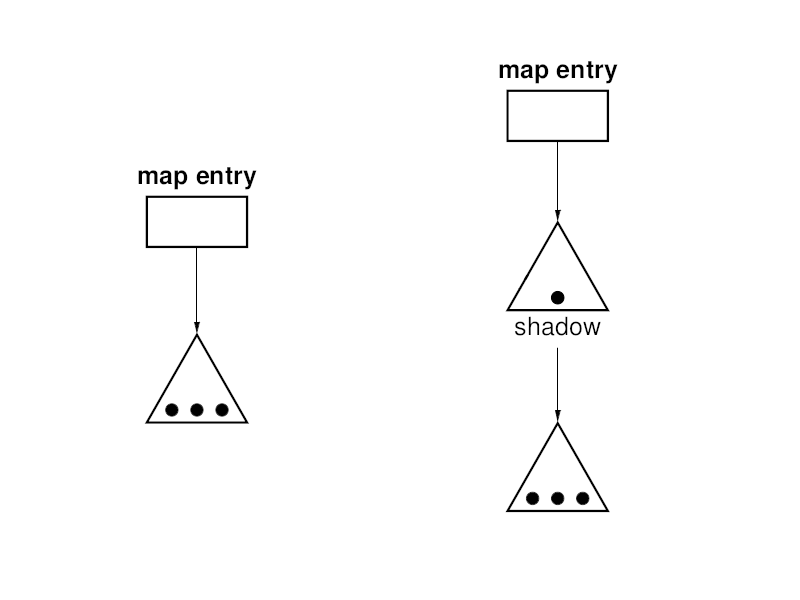
\includegraphics[scale=0.9]{copy-shadow.png}
  \caption{Creation of shadow VM object \cite{cranor}}
  \label{img:copy_shadow}
\end{figure}

We can observe that after some time there may emerge a \mintinline{c}{shadow object chains}.
The shadow objects is private for the process that owns it, therefore after the process has forked, there will possibly be
created a new shadow object that will reference the old one.
In every created shadow object in such chain there may still be some pages, that weren't modified yet and not transferred to the upper objects.
On the figure \ref{img:multiple_shadow_objs} there is an example of a simple VM object chain.
The first shadow VM object was created by a write to the private memory region by the parent process (before fork).
After forking, each process had written to some memory page and in result both processes had to create new shadow objects to hold their changes to the memory.

\begin{figure}[h]
  \centering
  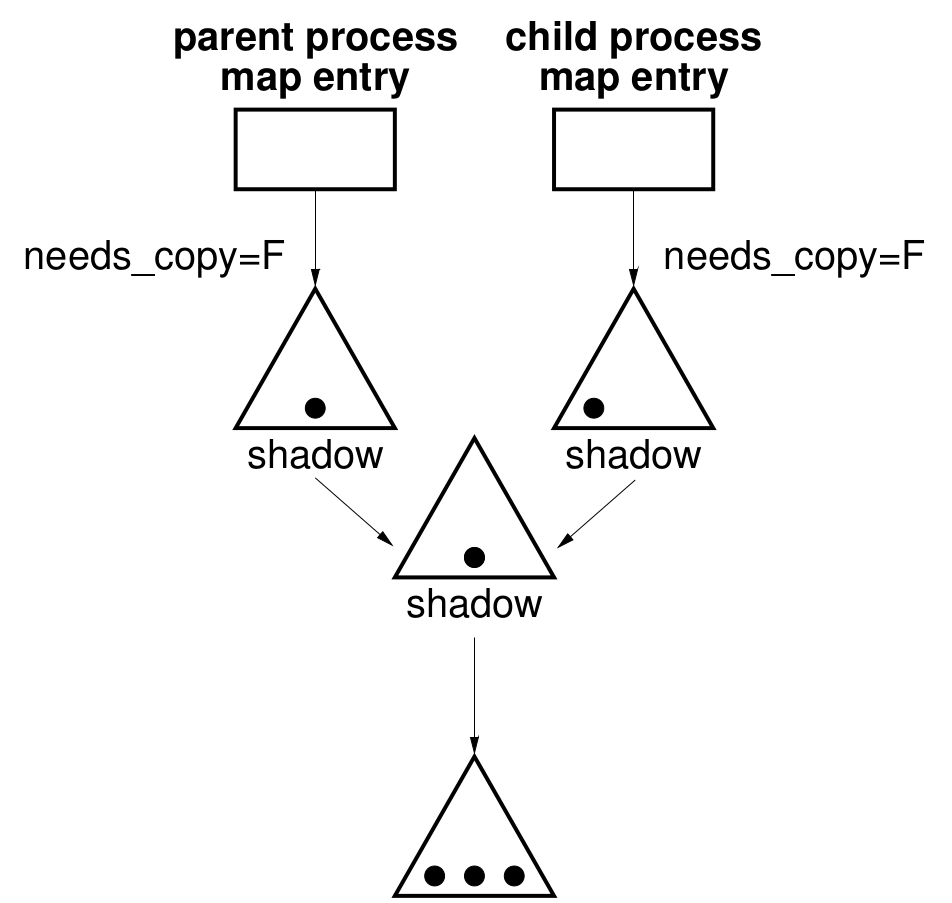
\includegraphics[scale=0.15]{multiple-shadow-objs.png}
  \caption{Two level shadow object chains \cite{cranor}}
  \label{img:multiple_shadow_objs}
\end{figure}

Because there are many levels of VM objects containing memory pages,
the page fault routine must search the entire VM object chain to locate a page in the VM~map.
This is necessary because the page may be in the lowest VM object, which is the first one created in the chain.
This process may take a long time since there is no limit to the length of the chain.

The VM object chain might be collapsed under certain circumstances.
In some cases, all pages in a shadow object have their copies in all objects above it.
To decide if an object can be removed from the chain after a page was copied to an upper VM object,
we have to pass the information about which page was copied down the chain.

The example shadow object chain that can be collapse is presented on figure \ref{img:collapse_shadow_chain}.
The only page that belongs to the object in the middle has its copy in the object above.
Such situation is usually encountered when the child process has exited and the parent is still using memory, so all of it has been copied to the upper shadow object.

\begin{figure}
  \centering
  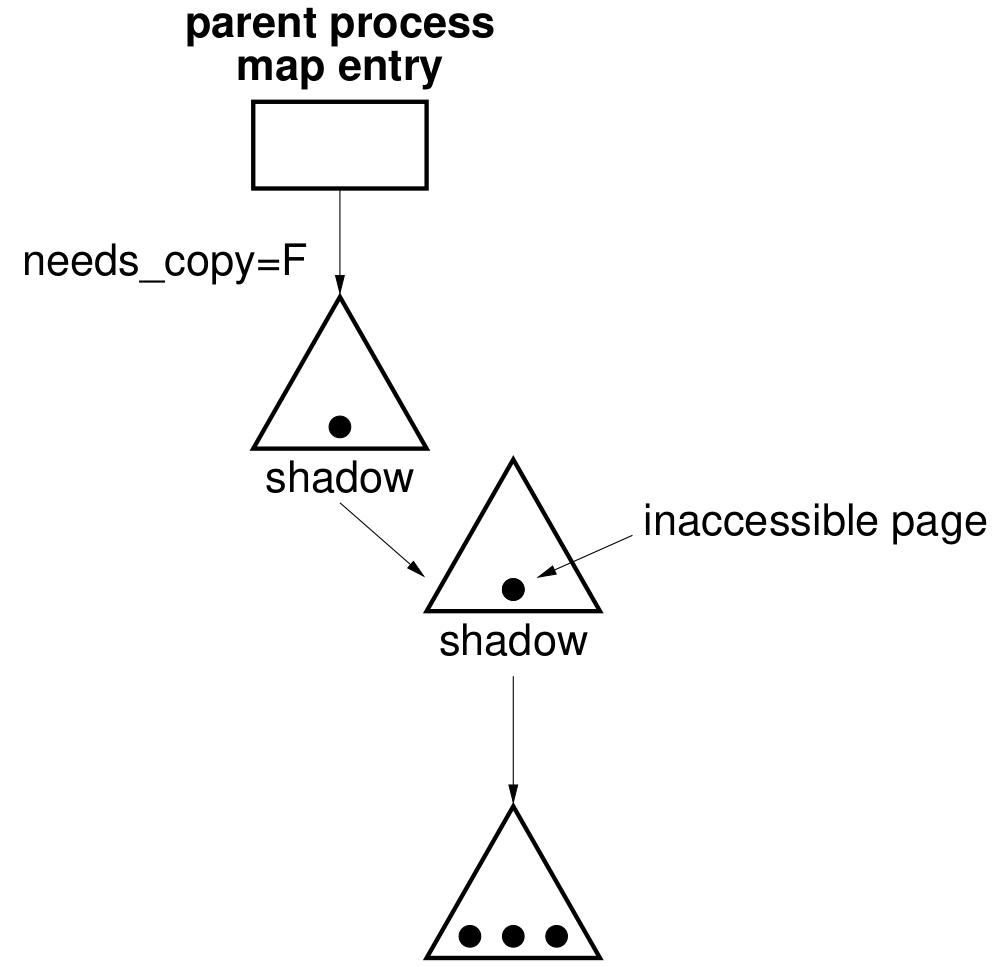
\includegraphics[scale=0.15]{collapse-shadow-chain.png}
  \caption{Shadow object chain that can be collapsed \cite{cranor}}
  \label{img:collapse_shadow_chain}
\end{figure}


\subsection{Summary of differences}

Most of the differences between UVM and BSD~VM are observed during the fork operation and the page fault routine.
These are the places which that strongly intervene with VM~map of the process.
On high level the differences are spotted due to the structure of VM~maps.
In UVM the structure is well defined and always has not more than two levels where pages could be stored.
In BSD~VM the structure might get much bigger, and harder to operate on due to possible long VM object chains.

The UVM system is also more concentrated on managing the anonymous memory.
There is more control over single anonymous pages, because they are described with separate structures designed with anonymous memory in mind.
This design makes it possible to implement new functions, that was not possible or hard to accomplish in old design.
In the original implementation of UVM there are three new operations, which were hard or impossible to implement in the old BSD~VM:

\begin{itemize}
  \item Page loan -- temporarily giving read-only access to some page to the kernel or other process.
  \item Page transfer -- transferring the page to the process VM~map from the kernel or other process.
  \item Map entry passing -- passing an VM~map entry to another process (e.g. the part of memory mapped file).
  \item Partial deallocation -- freeing the areas of anonymous memory that are no longer used (which wasn't possible in the BSD~VM).
\end{itemize}

The detailed comparison of these two implementation, as well as description of all implementation details of UVM and improvements
over the BSD~VM, is described in the Charles D. Cranor in his dissertation \cite{cranor}.
